\chapterimage{./Pictures/cover-gear}
\chapter{TP1 : Méthodes de classe et méthodes d'instance}
\textit{L’objectif de ce premier TP est de nous familiariser avec la notion de classe, notion essentielle de la programmation en Java, en nous faisant créer plusieurs classes illustrant une situation concrète et notamment d’insister sur la différence entre méthodes de classe et méthode d’instance.}

\section{Exercice 1 : Classe Ville}
\textit{L'objectif de cet exercice est de créer une classe Ville possédant un nom, une superficie et une population. Un constructeur par défaut ains qu'un constructeur prenant en paramètre les trois attributs cité précedemment ainsi que les accesseurs et mutateurs de chaques attributs seront ajoutés à la classe. Nous allons également surcharger la méthode toString() afin d'afficher la description d'une Ville.}
\inputminted[linenos,firstline=3,lastline=90]{java}{../sources/src/tp1/Ville.java}

\section{Exercice 2 : Classe Departement}
\textit{L'objectif de cet exercice est de créer une clase Département, permettant de regrouper plusieurs villes. Cette classes possèdera comme attributs, un nom, un numéro, un nombre de villes saisies et donc un tableau de Villes. Un constructeur sera ajouté à la classe ainsi qu'une méthode ajouterVille, permettant d'ajouter une Ville au tableau de Villes du Département. Nous allons également surcharger la méthode toString() afin d'afficher la description d'un département et ses villes qu'il contient.}
\inputminted[linenos,firstline=3,lastline=80]{java}{../sources/src/tp1/Departement.java}

\section{Exercice 3 : Classe Main}
\textit{L'objectif de cet exercice est de créer un classe Main contenant une méthode main dans laquelle nous allons instancier les différentes classes nécessaire au scénario proposé.}
\inputminted[linenos,firstline=3,lastline=29]{java}{../sources/src/tp1/Main.java}

\begin{figure}[H]
  \centering
  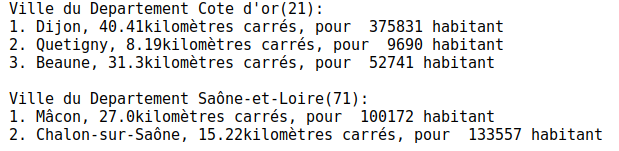
\includegraphics[width=400pt]{./tp/Pictures/tp1-execute}
  \caption{Exécution TP1}
  \label{Exécution TP1}
\end{figure}

\section{Exercice 4 : Attributs et méthodes de classe vs attributs et méthodes d'instances}
\textit{L'objectif de cet exercice est de manipulier le mot clef \mintinline{java}{static} afin différencier les membres de classe et les membres d'instance.}
On remarque que si l'on rajoute le mot clef \mintinline{java}{static} à l'attribut nom de la classe Département, toutes les instances de Département auront le même nom.

En effet le mot clef \mintinline{java}{static} permet de spécifier qu'un membre appartient à tout une classe plutôt qu'une instance, c'est à dire que seulement une instance d'attribut static sera existante même si l'on crée un centaine d'instance de la classe.

Les deux méthodes \mintinline{java}{estIdentiqueA(Ville v)} et \mintinline{java}{sontIdentiques(Ville v1, Ville v2)} permettent de comparer deux Ville.\\
On implémente ainsi ces méthodes :

\inputminted[linenos,firstline=59,lastline=70]{java}{../sources/src/tp1/Ville.java}

\begin{itemize}
  \item \mintinline{java}{estIdentiqueA(Ville v)} de comparer une instance de Ville depuis une autre instance de Ville.
  \item \mintinline{java}{sontIdentique(Ville v1, Ville v2)} permet de comparer deux instance de Ville depuis la classe Ville.
\end{itemize}

Nous allons faciliter la comparaison de deux instance en surchargeant la méthode \mintinline{java}{equals} ainsi que la méthode \mintinline{java}{hashCode} de la manière suivante :
\inputminted[linenos,firstline=72,lastline=89]{java}{../sources/src/tp1/Ville.java}
